\section{Results}
\label{sec:results}



\begin{table}[htbp!]
\caption{Predictions in the signal regions}
\centering
\begin{tabular}{c|c|c|c|c|c|}
\hline \hline
\MET bin & Uncertainty from MET shape & Uncertainty from mass shape & Total Pred. & Obs. & T5ZZ(1700) \\
\hline \hline
 $\MET[300,450]$ & $18.05 \pm 3.39$  & $0.98 \pm 0.11$ & $17.68 \pm 3.85$ & 15 & 0.24 & 0.75  \\ \hline 
 $\MET[450,600]$& $4 \pm 1.54$ & $0.86 \pm 0.16$ & $3.44\pm 1.47$ &  2  & 0.32 & 0.98 \\\hline
 $\MET[600,800]$&  $0.71 \pm 0.50$  &  $0.86 \pm 0.17$ & $0.61\pm 0.45$ &  1 & 2.13 & 4.34\\\hline
 $\MET[800,1000]$ & $18.05 \pm 3.39$  & $0.98 \pm 0.11$ & $17.68 \pm 3.85$ & 15 & 0.24 & 0.75  \\ \hline 
 $\MET>1000$& $4 \pm 1.54$ & $0.86 \pm 0.16$ & $3.44\pm 1.47$ &  2  & 0.32 & 0.98 \\\hline
\hline
\end{tabular}
\label{tab:DataPred}
\end{table}


\begin{figure}[htbp!]
  \begin{center}
    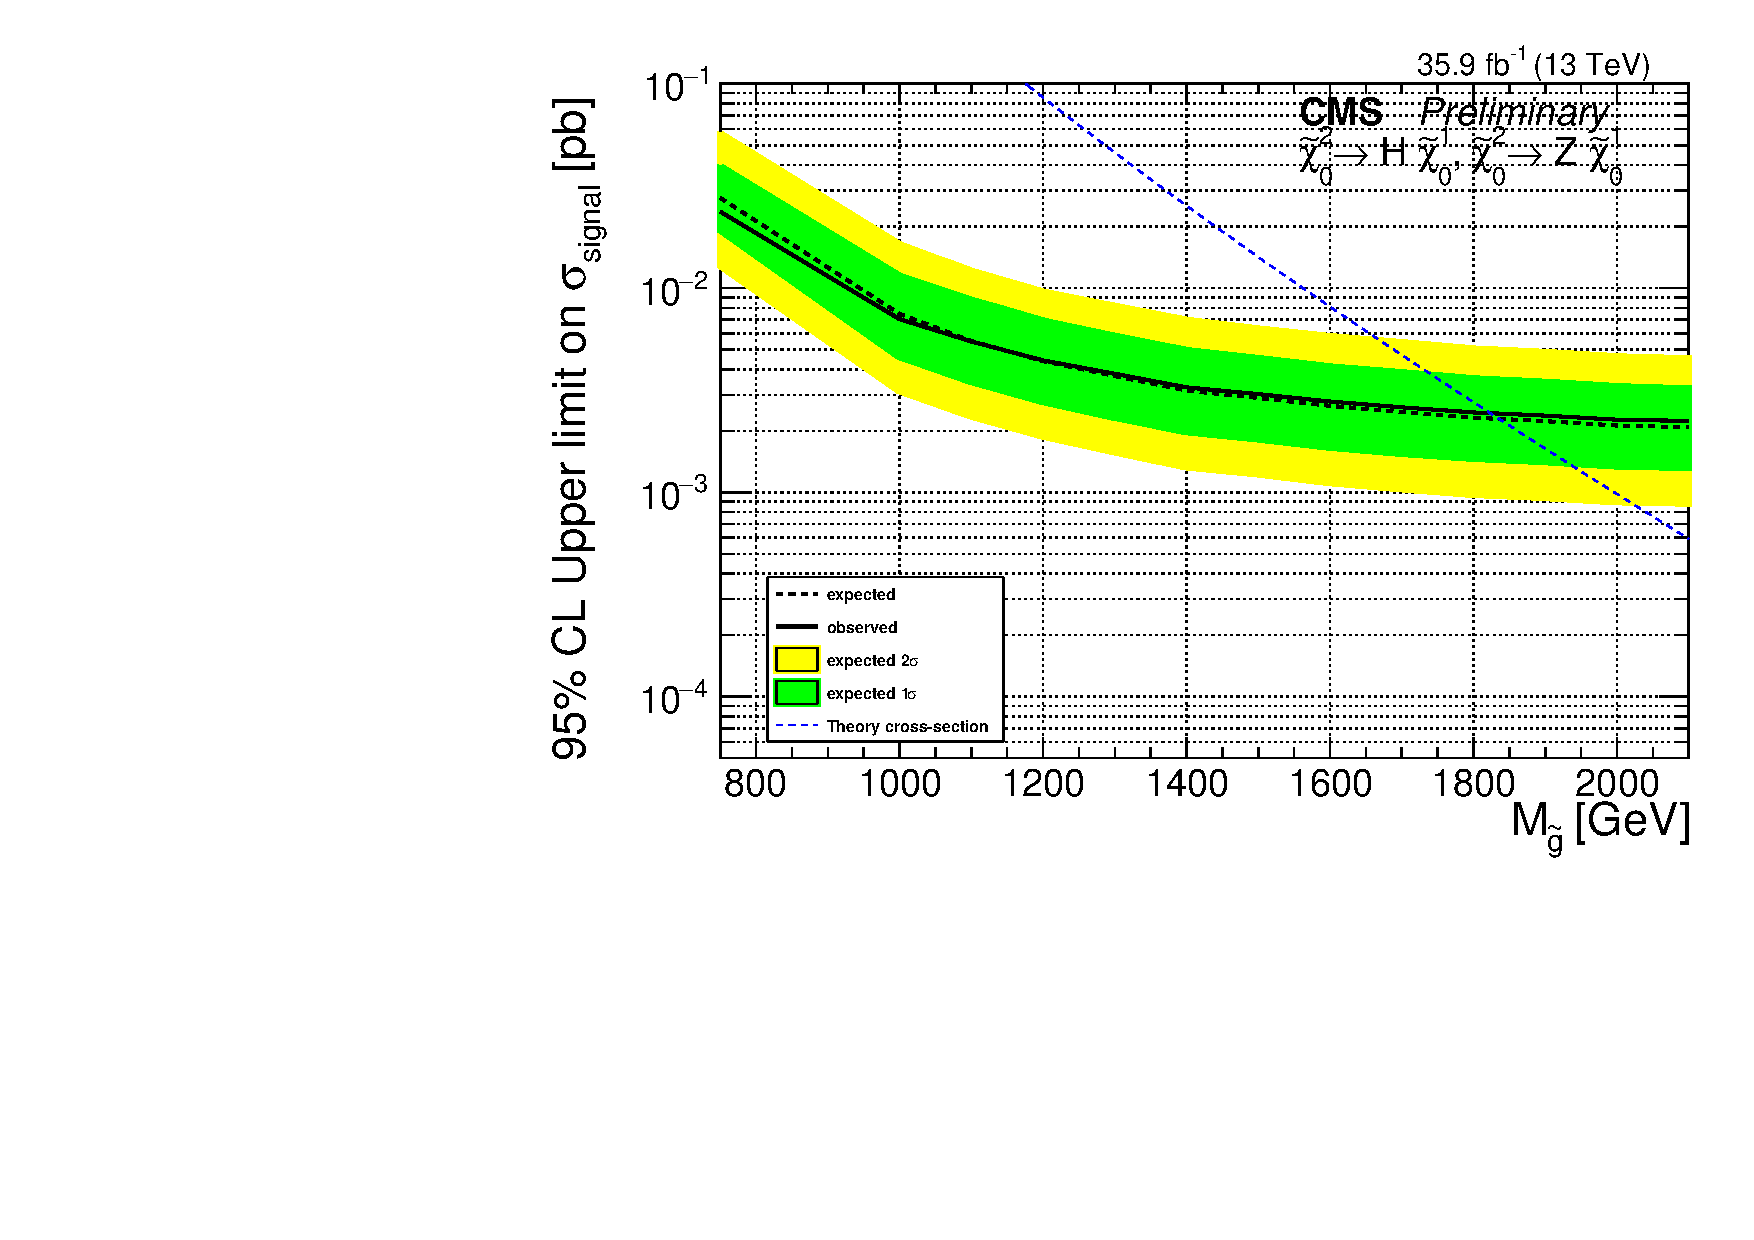
\includegraphics[width=0.6\linewidth]{plots/results/brazilT5HZResults.pdf}
    \caption{$95\%$ CL limit for the signal model considered in this analysis:  100$\%$ branching fraction to the Z boson
    }
    \label{fig:LimitsT5HH}
  \end{center}
\end{figure}

